\documentclass[10pt,conference,compsocconf]{IEEEtran}

%\usepackage{times}
%\usepackage{balance}
\usepackage{url}
\usepackage{graphicx}	% For figure environment
\usepackage{color}


\begin{document}
\title{Writing Scientific Papers and Software}

\author{
  Cheng Soon Ong\\
  Department of Computer Science, ETH Zurich, Switzerland
}

\maketitle

\begin{abstract}
  A critical part of scientific discovery is the
  communication of research findings to peers or the general public.
  Mastery of the process of scientific communication improves the
  visibility and impact of research. While this guide is a necessary
  tool for learning how to write in a manner suitable for publication
  at a scientific venue, it is by no means sufficient, on its own, to
  make its reader an accomplished writer. We also describe the rules
  for submission in the computational intelligence laboratory.
  This guide should be a
  starting point for further development of writing skills.
\end{abstract}

\section{Introduction}

Recommender systems have gained increasing popularity in the last 10-15 years, mainly due to their immediate market applications. The huge selection of products online offer retailers the opportunity to attract a wide-range of clients. However, it also means that users can no longer be expected to browse through everything available until they find the film, song or book they like the most. Good recommendations are key to both making the correct products available to the appropriate audience, but also to creating a unique, personalised experience which will attract new clients. These ideas are fundamental for many leading online businesses [ref netflix, ref amazon, ref something else].

In this paper, we concentrate on the collaborative-filtering approach to recommender systems, which relies on previous user experiences (ratings), rather than pre-defined user profile [some ref about the two types]. We use the Netflix dataset with ratings from 10000 users on 1000 films, which has driven a lot of the innovation in the area and allows us to compare our solutions to the state-of-the-art. 

Our main contributions are two-fold: we first combine latent factor models (SVD, SGD SVD, RBM) and neighbourhood models (user- and item-based kNN) to produce a robust recommender system which optimises the RMSE of predicted ratings on X[how many films] from Blaa to Bllaa. Second, we show that the addition of a more complex learning rate heuristic on stochastic gradient descent and restricted Boltzmann machines improves the score significantly, to X. 

In Section \ref{sec:models} we describe the idea and the implementation of our systems. We present the results from the local evaluation of the models and from the validation set on Kaggle in Section \ref{sec:results}. Finally, in Section \ref{sec:discussion} we interpret the improvements we achieved and discuss potential weaknesses and future work.



\section{Models and Methods}
\label{sec:models}
All work is done on the Netflix dataset provided for the project. The data is a collection of \textit{(user, film, rating)} tuples. For training, we have 1176953 ratings available. The online evaluation on Kaggle is performed on another 1176953 ratings. We were able to see the prediction accuracy on 50\% of that online dataset and our goal was to improve that as it is believed to be very similar to the other 50\% of the data.
\subsection{Data Model}

The provided dataset can be most naturally seen as an $N\times M$ matrix, with $N$ being the number of users ($N=~10000$), and $M$ the number of films ($M=1000$). If every user had rated every film, the matrix would have $10^7$ entries. However, in this realistic scenario, this is not the case and our matrix is quite sparse. From here stems the difficulty of the problem - we attempt to predict more than a million ratings based on a very incomplete dataset. 

There are two main views which yield different methods for tackling this problem.

\subsubsection*{\textbf{Latent factor models}} 

%{\color{red} Modify because of RBM} This approach tries to explain the ratings as influenced by a set of unknown (latent) factors. Both users and items can be characterized by these latent factors and they are represented as low-dimensional feature vectors in this latent feature space. The rating of a film is approximated by the dot product between the user and film feature vectors.
%
%The different methods then aim to infer the underlying film and user feature vectors from the available ratings, most successfully through matrix factorization techniques and approximations. We discuss Singular Value Decomposition and Stochastic Gradient Descent as particular examples of methods which follow this approach.
%
%We also discuss another latent factor model which is based on a different philosophy.

These models attempt to explain film ratings by users as being influenced by a set of unknown (also called \emph{latent}) factors.

One approach characterizes users and films by low-dimensional feature vectors in a latent feature space. The rating of a given film by a given user is then modeled by the dot product between the corresponding user and film feature vectors. The different methods then aim to infer the underlying film and user feature vectors from the available ratings, most successfully through matrix factorization techniques and approximations. As examples of this approach, we discuss Singular Value Decomposition and Stochastic Gradient Descent.

It is also possible to model missing ratings through neural networks which are composed by visible and latent units. In particular, we discuss Restricted Boltzmann Machines. At a high level, for each user-film pair whose rating is missing, the neural network learns a probability distribution over the possible ratings (1 to 5) from the known ratings. The prediction is then simply the expected value of this distribution.


\subsubsection*{\textbf{Neighbourhood-based models}} Another approach to the collaborative filtering problem is to view the ratings as features of either the users (user-based) or the films (item-based). In the former case, a user A is represented as a sparse feature vector of their ratings and we would base our prediction on other users who have rated those films similarly. In the latter scenario, we would use the similarity between the new film and the films already rated by A to estimate the new rating. Each film is a feature vector of all users' ratings. We review an implementation of both in the next subsection.

\subsection{Algorithms}
We investigated three algorithms which concentrate on solving the latent-factor model problem and two which work on the neighbourhood model:

\subsubsection*{\textbf{Singular Value Decomposition (SVD)}} Given the latent factor model described above, the rating matrix is produced by the multiplication of the users matrix and films matrix which are all on the same feature space. The most natural way to infer the users and films representation is using a matrix factorisation approach so SVD comes directly to mind[some refs here]. The main issue is that SVD works on full matrices and as mentioned above, this is not the case. Hence, we need to impute the missing values before we can proceed. This introduces noise and leads to sup-optimal results. We hope to minimize the noise and the overfitting by looking for a low-rank ($k$) approximation of the rating matrix. 

We experimented with input strategies, different number of latent features and values for $k$ using a local validation set. We concluded that the best results were accomplished using XX features and Equation \ref{eq:imputation} for imputation:

\begin{equation}
R_{ij}= 0.5\cdot \textnormal{AvgUser}[i] + 0.5\cdot \textnormal{AvgFilm}[j]
\label{eq:imputation}
\end{equation}

A missing rating of user $i$ for film $j$ is calculated as a linear combination of the average rating given by user $i$, $\textnormal{AvgUser}[i]$, and the average rating received by film $j$ from all other users, $\textnormal{AvgFilm}[j]$. If any of those values is missing due to a film with no ratings or user with no rated films, the other value is used.

We have used the Numpy built-in SVD algorithm for this. Despite the optimization strategies, we expect the results achieved with SVD to be suboptimal due to the large number of missing values, and the inaccuracy introduced by the imputation of those values. We use this algorithm as a baseline and we try to improve it with better strategies for matrix factorization or alternative approaches of finding the latent factor representation.

\subsubsection*{\textbf{Stochastic Gradient Descent (SGD) for SVD}} The main idea of the algorithm is to avoid the need of filling in the missing values in the $k$-rank approximation of the rating matrix. 

Instead of doing the standard SVD which requires a full matrix, we use only the available ratings in a Stochastic Gradient Descent method. The function we minimize is :

\begin{equation}
equation for SGD
\end{equation}

The approximation should be much more representative of the data as it only uses real ratings. The algorithm was very sensitive to hyper-parameters so those were optimized on both a local validation set and the online Kaggle score. 

\subsubsection*{\textbf{Restricted Boltzmann Machines (RBM's)}}

RBM's are neural networks consisting of a layer of visible units and a layer of hidden units. Each unit has a stochastic binary random variable associated with it. There may be undirected connections between hidden and visible units, but no hidden-hidden or visible-visible connections are allowed. Thus, an RBM takes the form of a bipartite graph, where each layer corresponds to a different bipartition. These networks are a restricted version of Boltzmann machines (hence the name), introduced in \cite{AHS85}.

Recently, RBM's have found applications in collaborative filtering, as illustrated in \cite{SMH07}. A very nice overview of RBM's for collaborative filtering can be found in \cite{L10}. Our approach is based on these two works, although there are some differences.

We first build an RBM with 5000 visible units $v^k_i$, for $k\in\{1,\dots,5\}$ and $i\in\{1,\dots,1000\}$, and $L$ hidden units $h_1,\dots, h_L$, where $L$ is a hyper-parameter of the algorithm. Furthermore, for each hidden unit $h_j$ we add connections to every visible unit $v^k_i$. Each connection between $h_j$ and $v^k_i$ has an associated weight $W^k_{ij}$. Each hidden unit $h_j$ has an associated bias $b_j$ and each visible unit $v^k_i$ has an associated bias $b^k_i$. Finally, each unit can be in state 0 or 1.

The probability that a given unit is turned on (i.e. its associated state is 1) is a logistic function of the states of the units it is connected to. In our case we have
\[
p(v^k_i=1|h)=\frac{\exp(b^k_i+\sum_{j=1}^L h_jW^k_{ij})}{\sum_{l=1}^{5}\exp(b^l_i+\sum_{j=1}^{L}h_jW^l_{ij})}
\]
and
\[
p(h_j=1|V)=\frac{1}{1+\exp(-b_j-\sum_{i=1}^{1000}\sum_{k=1}^{5}v^k_iW^k_{ij})}.
\]

To train our RBM, we divide the users into small batches. For each user $u$ in a batch, we set $v^k_i=1$ if and only if user $u$ gave rating $k$ to film $i$. We then compute $p_j=p(h_j=1|V)$ when $V$ is set according to each of the users in the batch and record $v^k_i$ and $p_j$ for each triple $(i,j,k)$.

After going through each batch, we update the weights and biases. The learning rules are
\[
\Delta W^k_{ij}=\lambda(<v^k_ih_j>^+-<v^k_ih_j>^-)
\]
\[
\Delta b^k_i = \lambda(<v^k_i>^+-<v^k_i>^-)
\]
\[
\Delta b_j = \lambda(<h_j>^+-<h_j>^-),
\]
where $\lambda$ is the learning rate, $<v^k_ih_j>^+$ is the average (over all users in the batch) of $v^k_i\cdot p_j$, $<v^k_i>^+$ is the average of $v^k_i$ and $<h_j>^+$ is the average of $p_j$. Furthermore, $<v^k_i>^-$ and analogous quantities correspond to averaged probabilities of finding the corresponding units turned on simultaneously  when the neural network is running at equilibrium. These quantities are hard to compute exactly, but they can be approximated via Gibbs sampling (see \cite{H02}). This procedure is especially simple for RBM's, since each layer (hidden and visible) can be alternately updated in parallel. In our algorithm we use a single step of Gibbs sampling. Increasing the number of steps had no effect on the prediction score of our RBM.

Note that we train only a single RBM. In \cite{SMH07}, the method presented consists of building a different RBM for each user, which all share the same weights and biases. In particular, they keep only connections from hidden units to visible units corresponding to observed ratings of a particular user.

The prediction algorithm is the same in our method and in \cite{SMH07} and \cite{L10}. Namely, for a fixed user $u$, we set $v^k_i=1$ if and only if user $u$ ranked film $i$ with rating $k$. We then compute $\hat{p}_j=p(h_j=1|V)$ for $j=1,\dots, L$. If we want to predict the rating of film $i$, we compute
\[
p(v^k_i=1|\hat{p})=\frac{\exp(b^k_i+\sum_{j=1}^L \hat{p}_jW^k_{ij})}{\sum_{l=1}^{5}\exp(b^l_i+\sum_{j=1}^{L}\hat{p}_jW^l_{ij})},
\]
for $k=1,\dots, 5$. This yields a probability distribution over the possible ratings for movie $i$. Our prediction is 
\[
\sum_{k=1}^{5}k\cdot p(v^k_i=1|\hat{p}),
\]
(i.e. the expected value of the distribution).

We make use of the built-in BernoulliRBM algorithm in sklearn to create our RBM and train it. Furthermore, we modified the source code to add an heuristic for the learning rate of the RBM, which improved its performance.

\subsubsection*{\textbf{User-based $k$-Nearest Neighbors}} User based neighborhood methods are considered one of the most intuitive methods for collaborative filtering. It consists of two steps. First, the algorithm identifies a subset of users $N(u)$ of size $k$ who share a similar taste with a certain user $u$. Second, In order to predict the rating of user $u$ for a particular movie $m$, the ratings of users in $N(u)$ who have rated movie $m$ are aggregated according to their similarity measure with user $u$ to estimate the rating of user $u$ to movie $m$. The similarity measure, which according to literature [xxx see msc thesis] was found to be the most accurate was the Pearson correlation measure. We denote the Pearson correlation between two users $u_1$ and $u_2$ by $w(u_1, u_2)$ and it is calculated as follows:
\begin{equation} \label{eqn:pearson}
\frac{\sum_{i \in C} (R(u_1, i) - \overline{R}_C(u_1))\cdot(R(u_2, i) - \overline{R}_C(u_2))}{\sqrt{\sum_{i \in C} (R(u_1, i) - \overline{R}_C(u_1))^2} \sqrt{\sum_{i \in C} (R(u_2, i) - \overline{R}_C(u_2))^2}}
\end{equation}

$C$ in the above equation is the set of co-rated items between users $u_1$ and $u_2$. $R(u,i)$ is the rating of user $u$ to movie $i$. $\overline{R}_C(u)$ is the average rating of user $u$ on the set of movies $C$. The higher the correlation, the more similar the two users $u_1$ and $u_2$. We also have to introduce another similarity measure named cosine-based similarity for reasons that will be apparent shortly. Cosine-based similarity computes the cosine of the angle between the two vectors corresponding to the co-rated items of two users. Each user $u_1$ and $u_2$ is represented by a vector of ratings of movies in the set $C$ of co-rated movies. Next we measure the cosine of the angle between these two vectors. The equation is as follows:
\begin{equation}
\frac{\overrightarrow{R_C}(u_1) \cdot {\overrightarrow{R_C}(u_2)}}{\|R_C(u_1)\| \|R_C(u_2)\|}
\end{equation}
The problem with such measure is that it does not take into account the fact that different users might have different scales for ratings. One user might consider a rating 3 as a high one and another user might consider a rating 3 to be low. Adjusting the cosine based similarity measure by subtracting the average of a user from all its ratings is surprisingly the same as the Pearson correlation measure [according to ...]. We introduced that measure since its implementation is already present in sklearn and allow for faster computation of the weight between different users. So we centered the ratings by subtracting the mean of all users from there respective ratings and used the built-in sklearn "pairwise\_distances" function using the cosine metric to compute the weights. After calculating the weights defining how similar two users are for all pairs of users. The best $k$ is chosen by calculating the error of the algorithm on a validation set for different values of $k$. Afterwards, to predict the unknown rating of a user $u$ for a particular movie $i$, we compute an averaged weighted sum of the ratings of the $k$ nearest neighbors to user $u$ as follows:
\begin{equation} \label{eqn:predict_user_based}
R(u,i) = \overline{R}(u) + \frac{\sum_{u_k \in N(u)} w(u,u_k)(R(u_k,i) - \overline{R}(u_k))}{\sum_{u_k \in N(u)} w(u,u_k)}
\end{equation}
where $N(u)$ is the set of the most similar $k$ users.
\\

\subsubsection*{\textbf{Item-based $k$-Nearest Neighbors}}  The item based kNN is considered to be the dual approach of the user based approach discussed above. Rather than finding similar users, the algorithm finds similar movies based on the ratings of all users. As above, a similarity measure such as the Pearson correlation is used to assess the similarity between each pair of movies. The set of users who rated movies $i$ and $j$ are used to measure as two vectors and the correlation is measured between them in a similar fashion as shown in equation (\ref{eqn:pearson}). in order to predict the rating of user $u$ for movie $i$, This is computed as follows:
\begin{equation}
R(u,i) = \overline{R}(i) + \frac{\sum_{j \in k\_R(u)} w(i,j)(R(u,j) - \overline{R}(j))}{\sum_{j \in k\_R(u)} w(i,j)}
\end{equation}
where $\overline{R}(i)$ is the average rating of movie $i$. $k\_R(u)$ is a set of movies for which we know the rating of user $u$. $w(i,j)$ is the similarity measure of movie $i$ and movie $j$. We can choose the size of the set $k\_R$ as we wish. 

\subsection{The bold driver heuristic} 
One of the biggest boosts to our score came from incorporating the bold driver heuristic for the learning rate in both SGD and RBM. This technique works as follows: Suppose we start with learning rate $\lambda$. After each epoch we compute the current error on the validation set and compare it with the error of the previous epoch. If the error increased from one epoch to the other, we decrease $\lambda$ to $d\lambda$, where $d\in[0,1]$ is a parameter we must set. On the other hand, if the error decreased, we increase $\lambda$ to $(1+c)\lambda$, where $c\geq 0$ is a parameter we must also set. Intuitively, the bold driver heuristic speeds up the convergence when we are going in the right direction and breaks quite sharply when we have missed a minimum and must turn around, so we do not miss it again by much. Thus, the bold driver heuristic adapts the learning rate to the surface we are trying to maneuver.

By playing with the parameters $\lambda$, $c$ and $d$ we can increase the performance of our methods significantly. In our case, for SGD, we obtained our best scores by setting $\lambda=0.001$, $c=0.05$, and $d=0.7$.

It is interesting to note that usual implementations of the bold driver heuristic also erase an update when it increases the error. In our implementation we opted to keep all such updates. Through experimentation we came to the conclusion that erasing ``bad" updates did not lead to any increase of performance for our methods. {\color{red} Should we test this further?}

\subsection{Parameter optimization and validation} 
The general protocol for training and testing followed the steps below:

\begin{enumerate}
\item Choose a random subset of the test samples for a local validation set if not already chosen. This was in most cases 5\% of the data, so xxxx samples and was only done by the first algorithm, so that all algorithms are trained on the same data.

\item Train each individual algorithm on the leftover test dataset. In some cases, such as in the item-base kNN, the validation set was used to automatically choose the optimal k in the predefined range. In the iterative algorithms like SGD and RBM, we used the validation set as an early indication on whether the error is really falling with every step. We would often optimise certain parameters using this validation data, such as number of features to user or algorithm iterations (see results for details).

\item Each algorithm generates predictions for the local validation set and the test set which would be uploaded on Kaggle.

\item The predictions from all algorithms are combined using linear regression. The regressor is trained on the predictions generated for local validation set for which we have ground truth. The coefficients which fit the results best are then used to generate a final prediction from all individual predictions for the online test dataset.

\end{enumerate}



\section{Results}
\label{sec:results}


\begin{figure}[tbp]
  \centering
  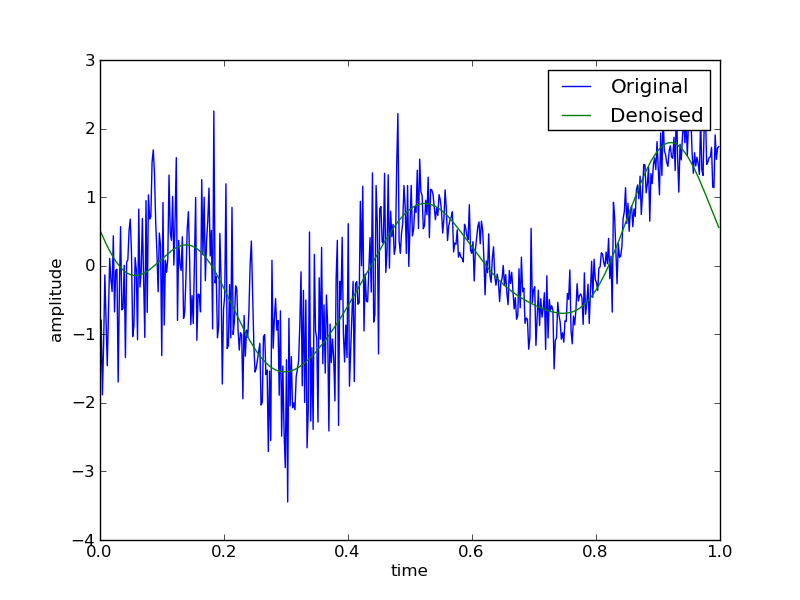
\includegraphics[width=\columnwidth]{denoised_signal_1d}
  \caption{Signal compression and denoising using the Fourier basis.}
  \label{fig:denoise-fourier}
\end{figure}
\begin{figure}[htbp]
  \centering
  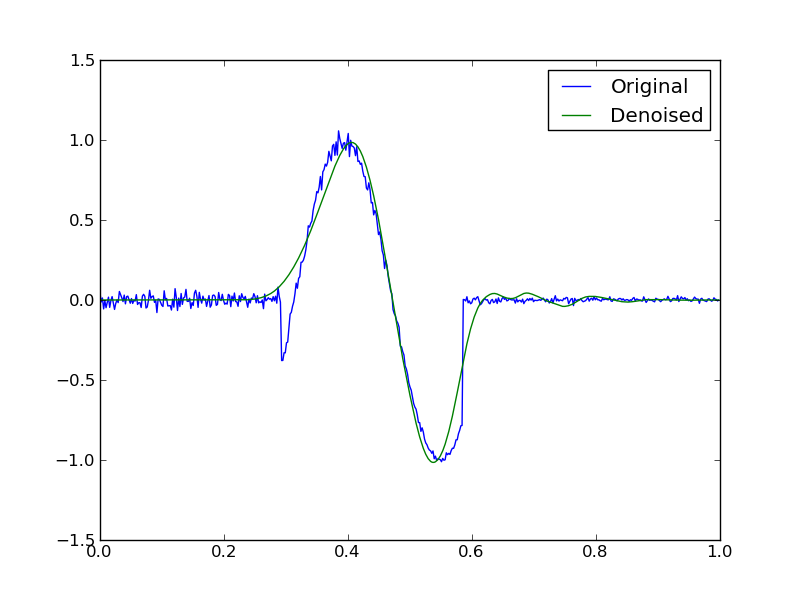
\includegraphics[width=\columnwidth]{local_wdenoised_1d}
  \caption{Signal compression and denoising using the Daubechies wavelet basis.}
  \label{fig:denoise-wavelet}
\end{figure}

Use examples and illustrations to clarify ideas and results. For
example, by comparing Figure~\ref{fig:denoise-fourier} and
Figure~\ref{fig:denoise-wavelet}, we can see the two different
situations where Fourier and wavelet basis perform well. 

\section{Discussion}
\label{sec:discussion}
The models and methods
section should describe what was
done to answer the research question, describe how it was done,
justify the experimental design, and
explain how the results were analyzed.

The model refers to the underlying mathematical model or structure which 
you use to describe your problem, or that your solution is based on. 
The methods on the other hand, are the algorithms used to solve the problem. 
In some cases, the suggested method directly solves the problem, without having it 
stated in terms of an underlying model. Generally though it is a better practice to have 
the model figured out and stated clearly, rather than presenting a method without specifying 
the model. In this case, the method can be more easily evaluated in the task of fitting 
the given data to the underlying model.

The methods part of this section, is not a step-by-step, directive,
protocol as you might see in your lab manual, but detailed enough such
that an interested reader can reproduce your
work~\cite{anderson04,wavelab}.

The methods section of a research paper provides the information by
which a study's validity is judged.
Therefore, it requires a clear and precise description of how an
experiment was done, and the rationale
for why specific experimental procedures were chosen.
It is usually helpful to
structure the methods section by~\cite{kallet04methods}:
\begin{enumerate}
\item Layout the model you used to describe the problem or the solution.
\item Describing the algorithms used in the study, briefly including
  details such as hyperparameter values (e.g. thresholds), and
  preprocessing steps (e.g. normalizing the data to have mean value of
  zero).
\item Explaining how the materials were prepared, for example the
  images used and their resolution.
\item Describing the research protocol, for example which examples
  were used for estimating the parameters (training) and which were
  used for computing performance.
\item Explaining how measurements were made and what
  calculations were performed. Do not reproduce the full source code in
  the paper, but explain the key steps.
\end{enumerate}

\subsection{Results}

Organize the results section based on the sequence of table and
figures you include. Prepare the tables and figures as soon as all
the data are analyzed and arrange them in the sequence that best
presents your findings in a logical way. A good strategy is to note,
on a draft of each table or figure, the one or two key results you
want to address in the text portion of the results.
The information from the figures is
summarized in Table~\ref{tab:fourier-wavelet}.

\begin{table*}[htbp]
  \centering
  \begin{tabular}[c]{|l||l|l|l|}
    \hline
    Basis&Support&Suitable signals&Unsuitable signals\\
    \hline
    Fourier&global&sine like&localized\\
    wavelet&local&localized&sine like\\
    \hline
  \end{tabular}
  \caption{Characteristics of Fourier and wavelet basis.}
  \label{tab:fourier-wavelet}
\end{table*}

When reporting computational or measurement results, always
report the mean (average value) along with a measure of variability
(standard deviation(s) or standard error of the mean).

\subsubsection{Installation}

There are various different packages available for processing \LaTeX{}
documents.
On Windows, use the Mik\TeX{} package (\url{http://miktex.org/}), and
on OSX use MacTeX
(\url{http://www.tug.org/mactex/2009/}). Alternatively, on OSX, you
can install the \texttt{tetex} package via
Fink\footnote{\url{http://www.finkproject.org/}} or 
Macports\footnote{\url{http://www.macports.org/}}.

\subsubsection{Compiling \LaTeX{}}
Your directory should contain at least 4 files, in addition to image
files. Images should be in \texttt{.png}, \texttt{.jpg} or
\texttt{.pdf} format.
\begin{itemize}
\item IEEEtran.cls
\item IEEEtran.bst
\item groupXX-submission.tex
\item groupXX-literature.bib
\end{itemize}
Note that you should replace groupXX with your chosen group name.
Then, from the command line, type:
\begin{verbatim}
$ pdflatex groupXX-submission
$ bibtex groupXX-literature
$ pdflatex groupXX-submission
$ pdflatex groupXX-submission
\end{verbatim}
This should give you a PDF document \texttt{groupXX-submission.pdf}.

\subsubsection{Equations}

There are three types of equations available: inline equations, for
example $y=mx + c$, which appear in the text, unnumbered equations
$$y=mx + c,$$
which are presented on a line on its own, and numbered equations
\begin{equation}
  \label{eq:linear}
  y = mx + c
\end{equation}
which you can refer to at a later point (Equation~(\ref{eq:linear})).

\subsubsection{Tables and Figures}

Tables and figures are ``floating'' objects, which means that the text
can flow around it.
Note
that \texttt{figure*} and \texttt{table*} cause the corresponding
figure or table to span both columns.


\subsection{Grading}

There are two different types of grading criteria applied to your
project, with the corresponding weights shown in brackets.
\begin{description}
\item[Competitive] \ \\
  The following criteria is scored based on your rank
  in comparison with the rest of the class.
  \begin{itemize}
  \item time taken for computation (10\%)
  \item average rank for all other criteria relevant to the task, for
    example reconstruction error and sparsity (20\%)
  \end{itemize}
  The ranks will then be converted on a linear scale into a grade
  between 4 and 6.
\item[Non-competitive] \ \\
  The following criteria is scored based on an
  evaluation by the teaching assistants.
  \begin{itemize}
  \item quality of paper (30\%)
  \item quality of implementation (20\%)
  \item creativity of solution (20\%)
  \end{itemize}
\end{description}

\subsection{Submission System}

The deadline for submitting your project report is Friday, 22 June
2012.
You need to submit:
\begin{itemize}
\item PDF of paper.
\item Archive (\texttt{.tar.gz} or \texttt{.zip}) of software. Please
  do not forget to include author information in the source archive.
\end{itemize}

\textbf{Important:} Please check the submission instructions on the webpage 
as it is the most updated instructions. 

\section{Summary}

The aim of a scientific paper is to convey the idea or discovery of
the researcher to the minds of the readers. The associated software
package provides the relevant details, which are often only briefly
explained in the paper, such that the research can be reproduced.
To write good papers, identify your key idea, make your contributions
explicit, and use examples and illustrations to describe the problems
and solutions.

\section*{Acknowledgements}
The author thanks Christian Sigg for his careful reading and helpful
suggestions.

\bibliographystyle{IEEEtran}
\bibliography{JKM-literature}
\end{document}
